\documentclass[journal,12pt,twocolumn]{IEEEtran}

\usepackage{setspace}
\usepackage{gensymb}
\singlespacing
\usepackage[cmex10]{amsmath}

\usepackage{amsthm}

\usepackage{mathrsfs}
\usepackage{txfonts}
\usepackage{stfloats}
\usepackage{bm}
\usepackage{cite}
\usepackage{cases}
\usepackage{subfig}

\usepackage{longtable}
\usepackage{multirow}

\usepackage{enumitem}
\usepackage{mathtools}
\usepackage{steinmetz}
\usepackage{tikz}
\usepackage{circuitikz}
\usepackage{verbatim}
\usepackage{tfrupee}
\usepackage[breaklinks=true]{hyperref}
\usepackage{graphicx}
\usepackage{tkz-euclide}

\usetikzlibrary{calc,math}
\usepackage{listings}
    \usepackage{color}                                            %%
    \usepackage{array}                                            %%
    \usepackage{longtable}                                        %%
    \usepackage{calc}                                             %%
    \usepackage{multirow}                                         %%
    \usepackage{hhline}                                           %%
    \usepackage{ifthen}                                           %%
    \usepackage{lscape}     
\usepackage{multicol}
\usepackage{chngcntr}

\DeclareMathOperator*{\Res}{Res}

\renewcommand\thesection{\arabic{section}}
\renewcommand\thesubsection{\thesection.\arabic{subsection}}
\renewcommand\thesubsubsection{\thesubsection.\arabic{subsubsection}}

\renewcommand\thesectiondis{\arabic{section}}
\renewcommand\thesubsectiondis{\thesectiondis.\arabic{subsection}}
\renewcommand\thesubsubsectiondis{\thesubsectiondis.\arabic{subsubsection}}


\hyphenation{op-tical net-works semi-conduc-tor}
\def\inputGnumericTable{}                                 %%

\lstset{
%language=C,
frame=single, 
breaklines=true,
columns=fullflexible
}
\begin{document}

\newcommand{\BEQA}{\begin{eqnarray}}
\newcommand{\EEQA}{\end{eqnarray}}
\newcommand{\define}{\stackrel{\triangle}{=}}
\bibliographystyle{IEEEtran}
\raggedbottom
\setlength{\parindent}{0pt}
\providecommand{\mbf}{\mathbf}
\providecommand{\pr}[1]{\ensuremath{\Pr\left(#1\right)}}
\providecommand{\qfunc}[1]{\ensuremath{Q\left(#1\right)}}
\providecommand{\sbrak}[1]{\ensuremath{{}\left[#1\right]}}
\providecommand{\lsbrak}[1]{\ensuremath{{}\left[#1\right.}}
\providecommand{\rsbrak}[1]{\ensuremath{{}\left.#1\right]}}
\providecommand{\brak}[1]{\ensuremath{\left(#1\right)}}
\providecommand{\lbrak}[1]{\ensuremath{\left(#1\right.}}
\providecommand{\rbrak}[1]{\ensuremath{\left.#1\right)}}
\providecommand{\cbrak}[1]{\ensuremath{\left\{#1\right\}}}
\providecommand{\lcbrak}[1]{\ensuremath{\left\{#1\right.}}
\providecommand{\rcbrak}[1]{\ensuremath{\left.#1\right\}}}
\theoremstyle{remark}
\newtheorem{rem}{Remark}
\newcommand{\sgn}{\mathop{\mathrm{sgn}}}
\providecommand{\abs}[1]{\vert#1\vert}
\providecommand{\res}[1]{\Res\displaylimits_{#1}} 
\providecommand{\norm}[1]{\lVert#1\rVert}
%\providecommand{\norm}[1]{\lVert#1\rVert}
\providecommand{\mtx}[1]{\mathbf{#1}}
\providecommand{\mean}[1]{E[ #1 ]}
\providecommand{\fourier}{\overset{\mathcal{F}}{ \rightleftharpoons}}
%\providecommand{\hilbert}{\overset{\mathcal{H}}{ \rightleftharpoons}}
\providecommand{\system}{\overset{\mathcal{H}}{ \longleftrightarrow}}
	%\newcommand{\solution}[2]{\textbf{Solution:}{#1}}
\newcommand{\solution}{\noindent \textbf{Solution: }}
\newcommand{\cosec}{\,\text{cosec}\,}
\providecommand{\dec}[2]{\ensuremath{\overset{#1}{\underset{#2}{\gtrless}}}}
\newcommand{\myvec}[1]{\ensuremath{\begin{pmatrix}#1\end{pmatrix}}}
\newcommand{\mydet}[1]{\ensuremath{\begin{vmatrix}#1\end{vmatrix}}}
\numberwithin{equation}{subsection}
\makeatletter
\@addtoreset{figure}{problem}
\makeatother
\let\StandardTheFigure\thefigure
\let\vec\mathbf
\renewcommand{\thefigure}{\theproblem}
\def\putbox#1#2#3{\makebox[0in][l]{\makebox[#1][l]{}\raisebox{\baselineskip}[0in][0in]{\raisebox{#2}[0in][0in]{#3}}}}
     \def\rightbox#1{\makebox[0in][r]{#1}}
     \def\centbox#1{\makebox[0in]{#1}}
     \def\topbox#1{\raisebox{-\baselineskip}[0in][0in]{#1}}
     \def\midbox#1{\raisebox{-0.5\baselineskip}[0in][0in]{#1}}
\vspace{3cm}
\title{AI1103-Assignment 3}
\author{Name : Ayush Jha \\ Roll Number: CS20BTECH11006}
\maketitle
\newpage
\bigskip
\renewcommand{\thefigure}{\theenumi}
\renewcommand{\thetable}{\theenumi}
Download all python codes from 
\begin{lstlisting}
https://github.com/ayushjha2612/AI11003/tree/main/Assignment3/Codes
\end{lstlisting}
%
and latex-tikz codes from 
%
\begin{lstlisting}
https://github.com/ayushjha2612/AI11003/tree/main/Assignment3
\end{lstlisting}
\section*{GATE Problem 34}
Let X and Y be two statistically independent random variables uniformly distributed in the range (-1, 1) and (-2, 1) respectively. Let $Z = X +Y$ , then the probability that $[Z \leq -2]$ is \\
(A) zero         \hfill  (B) $\dfrac{1}{6}$  \hfill
(C)$\dfrac{1}{3}$      \hfill       (D)$\dfrac{1}{12}$  
\section*{Answer}
Option (D) $\dfrac{1}{12}$
\section*{Solution}
X and Y are two independent random variables. \\
The range of X is $-1 \leq X \leq 1$ and the range of Y is $-2 \leq X \leq 1$ .\\ 
As it is a uniform distribution we have, 
\begin{equation}
    \Pr\brak{-1 \leq X \leq 0} = \Pr\brak{0 \leq X \leq 1}
\end{equation}
X is distributed in the range(-1,1) which implies that
\begin{align}
    \Pr\brak{-1 \leq X \leq 0} + \Pr\brak{0 \leq X \leq 1}= 1 \\
 2 \times \Pr\brak{-1 \leq X \leq 0} = 1
\end{align}

Therefore we have,
\begin{equation}
    \Pr\brak{-1 \leq X \leq 0} = \dfrac{1}{2}
\end{equation}
Similarly random variable Y is distributed in the range(-2 ,1)
$$\Pr\brak{-2 \leq Y \leq -1}=\Pr\brak{-1 \leq Y \leq 0} = \Pr\brak{0 \leq Y \leq 1} $$
And sum of these three probabilities is 1
Therefore we have,
\begin{align}
    3 \times \Pr\brak{-2 \leq Y \leq-1} = 1  \\
     \Pr\brak{-2 \leq Y \leq-1} = \dfrac{1}{3}
\end{align}
Now we have another random variable Z, which is defined as 
\begin{equation}
    Z = X + Y
\end{equation}
We need to find $\Pr\brak{Z \leq -2}$ 
\begin{equation}
    Z \leq 2 \implies X+Y \leq 2
\end{equation}
When the random variable, X lies in the range (-1,0) and Y lies in the range(-2,-1) we have that Z lies in the range (-3,-1). \\
As X and Y are independent random variables we have that
\begin{equation}
    \Pr\brak{XY} = \Pr\brak{X} \times  \Pr\brak{Y}
\end{equation}
Therefore we have,
\begin{align}
    \Pr\brak{-3 \leq Z \leq -1} &= \Pr\brak{(-2 \leq Y \leq -1)(-1 \leq X \leq 0)} \\
    &=  \dfrac{1}{3}  \times \dfrac{1}{2}  \\
    &= \dfrac{1}{6}
\end{align}
As it is a uniform distribution,
\begin{equation}
     \Pr\brak{-3 \leq Z \leq -2}=  \Pr\brak{-2 \leq Z \leq -1}
\end{equation}
Which gives us that,
\begin{equation}
     \Pr\brak{-3 \leq Z \leq -2}=  \dfrac{1}{12}
\end{equation}
So $\Pr\brak{ Z \leq -2}=  \dfrac{1}{12}$ i.e. option (D). \\
The theory vs simulation plot can be viewed at figure \ref{Theory VS simulation plot}. 

\begin{figure}[h!]
    \centering
    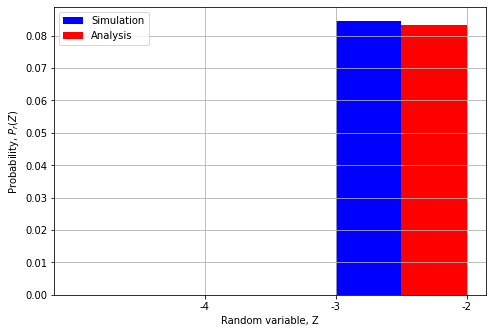
\includegraphics[width=11cm]{Assignment_3.png}
    \caption{Theory VS Simulation plot}
    \label{Theory VS simulation plot}
\end{figure}
\end{document}